%
% 6.006 problem set 4 solutions template
%
\documentclass[12pt,twoside]{article}

\newcommand{\name}{}

\usepackage{amssymb}
\usepackage{amsmath}
\usepackage{graphicx}
\usepackage{latexsym}
\usepackage{times,url}
\usepackage{cprotect}
\usepackage{listings}
\usepackage{graphicx}
\usepackage[table]{xcolor}
\usepackage[letterpaper]{geometry}
\usepackage{tikz-qtree}
\usepackage{enumerate}

\newcommand{\profs}{Instructors: Zachary Abel, Erik Demaine, Jason Ku}
\newcommand{\subj}{6.006}
\newcommand{\ttt}[1]{{\tt\small #1}}

\definecolor{dkgreen}{rgb}{0,0.6,0}
\definecolor{gray}{rgb}{0.5,0.5,0.5}
\definecolor{mauve}{rgb}{0.58,0,0.82}

\lstset{
  language=Python,
  aboveskip=1pc,
  belowskip=1pc,
  basicstyle={\footnotesize\ttfamily},
  numbers=left,
  showstringspaces=false,
  numberstyle=\tiny\color{gray},
  keywordstyle=\color{blue},
  commentstyle=\color{dkgreen},
  stringstyle=\color{mauve},
}

\tikzset{
  % every node/.style={minimum width=2em,draw,circle},
  % level 1/.style={sibling distance=2cm},
  level distance=1cm,
  edge from parent/.style=
  {draw,edge from parent path={(\tikzparentnode) -- (\tikzchildnode)}},
}

\newif\ifHideSolutions
\newcommand{\solution}[1]{\color{dkgreen}\textbf{Solution: }#1\color{black}}
\newcommand{\rubric}[1]{\color{dkgreen}{\bf Rubric:} #1\color{black}}

% \HideSolutionsfalse
% \ifHideSolutions
%   \renewcommand{\solution}[1]{}
%   \renewcommand{\rubric}[1]{}
% \fi

\newlength{\toppush}
\setlength{\toppush}{2\headheight}
\addtolength{\toppush}{\headsep}

\newcommand{\htitle}[2]{\noindent\vspace*{-\toppush}\newline\parbox{6.5in}
{\textit{Introduction to Algorithms: 6.006}\hfill\name\newline
Massachusetts Institute of Technology \hfill #2\newline
\profs\hfill #1 \vspace*{-.5ex}\newline
\mbox{}\hrulefill\mbox{}}\vspace*{1ex}\mbox{}\newline
\begin{center}{\Large\bf #1}\end{center}}

\newcommand{\handout}[2]{\thispagestyle{empty}
 \markboth{#1}{#1}
 \pagestyle{myheadings}\htitle{#1}{#2}}

\newcommand{\lecture}[3]{\thispagestyle{empty}
 \markboth{Lecture #1: #2}{Lecture #1: #2}
 \pagestyle{myheadings}\htitle{Lecture #1: #2}{#3}}

\newcommand{\htitlewithouttitle}[2]{\noindent\vspace*{-\toppush}\newline\parbox{6.5in}
{\textit{Introduction to Algorithms}\hfill#2\newline
Massachusetts Institute of Technology \hfill 6.006\newline
\profs\hfill Handout #1\vspace*{-.5ex}\newline
\mbox{}\hrulefill\mbox{}}\vspace*{1ex}\mbox{}\newline}

\newcommand{\handoutwithouttitle}[2]{\thispagestyle{empty}
 \markboth{Handout \protect\ref{#1}}{Handout \protect\ref{#1}}
 \pagestyle{myheadings}\htitlewithouttitle{\protect\ref{#1}}{#2}}

\newcommand{\exam}[2]{% parameters: exam name, date
 \thispagestyle{empty}
 \markboth{\hspace{1cm}\subj\ #1\hspace{1in}Name\hrulefill\ \ }%
          {\subj\ #1\hspace{1in}Name\hrulefill\ \ }
 \pagestyle{myheadings}\examtitle{#1}{#2}
 \renewcommand{\theproblem}{Problem \arabic{problemnum}}
}
\newcommand{\examsolutions}[3]{% parameters: handout, exam name, date
 \thispagestyle{empty}
 \markboth{Handout \protect\ref{#1}: #2}{Handout \protect\ref{#1}: #2}
% \pagestyle{myheadings}\htitle{\protect\ref{#1}}{#2}{#3}
 \pagestyle{myheadings}\examsolutionstitle{\protect\ref{#1}} {#2}{#3}
 \renewcommand{\theproblem}{Problem \arabic{problemnum}}
}
\newcommand{\examsolutionstitle}[3]{\noindent\vspace*{-\toppush}\newline\parbox{6.5in}
{\textit{Introduction to Algorithms}\hfill#3\newline
Massachusetts Institute of Technology \hfill 6.006\newline
%Singapore-MIT Alliance \hfill SMA5503\newline
\profs\hfill Handout #1\vspace*{-.5ex}\newline
\mbox{}\hrulefill\mbox{}}\vspace*{1ex}\mbox{}\newline
\begin{center}{\Large\bf #2}\end{center}}

\newcommand{\takehomeexam}[2]{% parameters: exam name, date
 \thispagestyle{empty}
 \markboth{\subj\ #1\hfill}{\subj\ #1\hfill}
 \pagestyle{myheadings}\examtitle{#1}{#2}
 \renewcommand{\theproblem}{Problem \arabic{problemnum}}
}

\makeatletter
\newcommand{\exambooklet}[2]{% parameters: exam name, date
 \thispagestyle{empty}
 \markboth{\subj\ #1}{\subj\ #1}
 \pagestyle{myheadings}\examtitle{#1}{#2}
 \renewcommand{\theproblem}{Problem \arabic{problemnum}}
 \renewcommand{\problem}{\newpage
 \item \let\@currentlabel=\theproblem
 \markboth{\subj\ #1, \theproblem}{\subj\ #1, \theproblem}}
}
\makeatother


\newcommand{\examtitle}[2]{\noindent\vspace*{-\toppush}\newline\parbox{6.5in}
{\textit{Introduction to Algorithms}\hfill#2\newline
Massachusetts Institute of Technology \hfill 6.006 Fall 2018\newline
%Singapore-MIT Alliance \hfill SMA5503\newline
\profs\hfill #1\vspace*{-.5ex}\newline
\mbox{}\hrulefill\mbox{}}\vspace*{1ex}\mbox{}\newline
\begin{center}{\Large\bf #1}\end{center}}

\newcommand{\grader}[1]{\hspace{1cm}\textsf{\textbf{#1}}\hspace{1cm}}

\newcommand{\points}[1]{[#1 points]\ }
\newcommand{\parts}[1]
{
  \ifnum#1=1
  (1 part)
  \else
  (#1 parts)
  \fi
  \ 
}

\newcommand{\bparts}{\begin{problemparts}}
\newcommand{\eparts}{\end{problemparts}}
\newcommand{\ppart}{\problempart}

%\newcommand{\lg} {lg\ }

\setlength{\oddsidemargin}{0pt}
\setlength{\evensidemargin}{0pt}
\setlength{\textwidth}{6.5in}
\setlength{\topmargin}{0in}
\setlength{\textheight}{8.5in}


\newcommand{\Spawn}{{\bf spawn} }
\newcommand{\Sync}{{\bf sync}}

\renewcommand{\cases}[1]{\left\{ \begin{array}{ll}#1\end{array}\right.}
\newcommand{\cif}[1]{\mbox{if $#1$}}
\newcommand{\cwhen}[1]{\mbox{when $#1$}}

\newcounter{problemnum}
\newcommand{\theproblem}{Problem \theproblemsetnum-\arabic{problemnum}}
\newenvironment{problems}{
        \begin{list}{{\bf \theproblem. \hspace*{0.5em}}}
        {\setlength{\leftmargin}{0em}
         \setlength{\rightmargin}{0em}
         \setlength{\labelwidth}{0em}
         \setlength{\labelsep}{0em}
         \usecounter{problemnum}}}{\end{list}}
\makeatletter
\newcommand{\problem}[1][{}]{\item \let\@currentlabel=\theproblem \textbf{#1}}
\makeatother

\newcounter{problempartnum}[problemnum]
\newenvironment{problemparts}{
        \begin{list}{{\bf (\alph{problempartnum})}}
        {\setlength{\leftmargin}{2.5em}
         \setlength{\rightmargin}{2.5em}
         \setlength{\labelsep}{0.5em}}}{\end{list}}
\newcommand{\problempart}{\addtocounter{problempartnum}{1}\item}

\newenvironment{truefalseproblemparts}{
        \begin{list}{{\bf (\alph{problempartnum})\ \ \ T\ \ F\hfil}}
        {\setlength{\leftmargin}{4.5em}
         \setlength{\rightmargin}{2.5em}
         \setlength{\labelsep}{0.5em}
         \setlength{\labelwidth}{4.5em}}}{\end{list}}

\newcounter{exercisenum}
\newcommand{\theexercise}{Exercise \theproblemsetnum-\arabic{exercisenum}}
\newenvironment{exercises}{
        \begin{list}{{\bf \theexercise. \hspace*{0.5em}}}
        {\setlength{\leftmargin}{0em}
         \setlength{\rightmargin}{0em}
         \setlength{\labelwidth}{0em}
         \setlength{\labelsep}{0em}
        \usecounter{exercisenum}}}{\end{list}}
\makeatletter
\newcommand{\exercise}{\item \let\@currentlabel=\theexercise}
\makeatother

\newcounter{exercisepartnum}[exercisenum]
%\newcommand{\problem}[1]{\medskip\mbox{}\newline\noindent{\bf Problem #1.}\hspace*{1em}}
%\newcommand{\exercise}[1]{\medskip\mbox{}\newline\noindent{\bf Exercise #1.}\hspace*{1em}}

\newenvironment{exerciseparts}{
        \begin{list}{{\bf (\alph{exercisepartnum})}}
        {\setlength{\leftmargin}{2.5em}
         \setlength{\rightmargin}{2.5em}
         \setlength{\labelsep}{0.5em}}}{\end{list}}
\newcommand{\exercisepart}{\addtocounter{exercisepartnum}{1}\item}


% Macros to make captions print with small type and 'Figure xx' in bold.
\makeatletter
\def\fnum@figure{{\bf Figure \thefigure}}
\def\fnum@table{{\bf Table \thetable}}
\let\@mycaption\caption
%\long\def\@mycaption#1[#2]#3{\addcontentsline{\csname
%  ext@#1\endcsname}{#1}{\protect\numberline{\csname 
%  the#1\endcsname}{\ignorespaces #2}}\par
%  \begingroup
%    \@parboxrestore
%    \small
%    \@makecaption{\csname fnum@#1\endcsname}{\ignorespaces #3}\par
%  \endgroup}
%\def\mycaption{\refstepcounter\@captype \@dblarg{\@mycaption\@captype}}
%\makeatother
\let\mycaption\caption
%\newcommand{\figcaption}[1]{\mycaption[]{#1}}

\newcounter{totalcaptions}
\newcounter{totalart}

\newcommand{\figcaption}[1]{\addtocounter{totalcaptions}{1}\caption[]{#1}}

% \psfigures determines what to do for figures:
%       0 means just leave vertical space
%       1 means put a vertical rule and the figure name
%       2 means insert the PostScript version of the figure
%       3 means put the figure name flush left or right
\newcommand{\psfigures}{0}
\newcommand{\spacefigures}{\renewcommand{\psfigures}{0}}
\newcommand{\rulefigures}{\renewcommand{\psfigures}{1}}
\newcommand{\macfigures}{\renewcommand{\psfigures}{2}}
\newcommand{\namefigures}{\renewcommand{\psfigures}{3}}

\newcommand{\figpart}[1]{{\bf (#1)}\nolinebreak[2]\relax}
\newcommand{\figparts}[2]{{\bf (#1)--(#2)}\nolinebreak[2]\relax}


\macfigures     % STATE

% When calling \figspace, make sure to leave a blank line afterward!!
% \widefigspace is for figures that are more than 28pc wide.
\newlength{\halffigspace} \newlength{\wholefigspace}
\newlength{\figruleheight} \newlength{\figgap}
\newcommand{\setfiglengths}{\ifnum\psfigures=1\setlength{\figruleheight}{\hruleheight}\setlength{\figgap}{1em}\else\setlength{\figruleheight}{0pt}\setlength{\figgap}{0em}\fi}
\newcommand{\figspace}[2]{\ifnum\psfigures=0\leavefigspace{#1}\else%
\setfiglengths%
\setlength{\wholefigspace}{#1}\setlength{\halffigspace}{.5\wholefigspace}%
\rule[-\halffigspace]{\figruleheight}{\wholefigspace}\hspace{\figgap}#2\fi}
\newlength{\widefigspacewidth}
% Make \widefigspace put the figure flush right on the text page.
\newcommand{\widefigspace}[2]{
\ifnum\psfigures=0\leavefigspace{#1}\else%
\setfiglengths%
\setlength{\widefigspacewidth}{28pc}%
\addtolength{\widefigspacewidth}{-\figruleheight}%
\setlength{\wholefigspace}{#1}\setlength{\halffigspace}{.5\wholefigspace}%
\makebox[\widefigspacewidth][r]{#2\hspace{\figgap}}\rule[-\halffigspace]{\figruleheight}{\wholefigspace}\fi}
\newcommand{\leavefigspace}[1]{\setlength{\wholefigspace}{#1}\setlength{\halffigspace}{.5\wholefigspace}\rule[-\halffigspace]{0em}{\wholefigspace}}

% Commands for including figures with macpsfig.
% To use these commands, documentstyle ``macpsfig'' must be specified.
\newlength{\macfigfill}
\makeatother
\newlength{\bbx}
\newlength{\bby}
\newcommand{\macfigure}[5]{\addtocounter{totalart}{1}
\ifnum\psfigures=2%
\setlength{\bbx}{#2}\addtolength{\bbx}{#4}%
\setlength{\bby}{#3}\addtolength{\bby}{#5}%
\begin{flushleft}
\ifdim#4>28pc\setlength{\macfigfill}{#4}\addtolength{\macfigfill}{-28pc}\hspace*{-\macfigfill}\fi%
\mbox{\psfig{figure=./#1.ps,%
bbllx=#2,bblly=#3,bburx=\bbx,bbury=\bby}}
\end{flushleft}%
\else\ifdim#4>28pc\widefigspace{#5}{#1}\else\figspace{#5}{#1}\fi\fi}
\makeatletter

\newlength{\savearraycolsep}
\newcommand{\narrowarray}[1]{\setlength{\savearraycolsep}{\arraycolsep}\setlength{\arraycolsep}{#1\arraycolsep}}
\newcommand{\normalarray}{\setlength{\arraycolsep}{\savearraycolsep}}

\newcommand{\hint}{{\em Hint:\ }}

% Macros from /th/u/clr/mac.tex

\newcommand{\set}[1]{\left\{ #1 \right\}}
\newcommand{\abs}[1]{\left| #1\right|}
\newcommand{\card}[1]{\left| #1\right|}
\newcommand{\floor}[1]{\left\lfloor #1 \right\rfloor}
\newcommand{\ceil}[1]{\left\lceil #1 \right\rceil}
\newcommand{\ang}[1]{\ifmmode{\left\langle #1 \right\rangle}
   \else{$\left\langle${#1}$\right\rangle$}\fi}
        % the \if allows use outside mathmode,
        % but will swallow following space there!
\newcommand{\paren}[1]{\left( #1 \right)}
\newcommand{\bracket}[1]{\left[ #1 \right]}
\newcommand{\prob}[1]{\Pr\left\{ #1 \right\}}
\newcommand{\Var}{\mathop{\rm Var}\nolimits}
\newcommand{\expect}[1]{{\rm E}\left[ #1 \right]}
\newcommand{\expectsq}[1]{{\rm E}^2\left[ #1 \right]}
\newcommand{\variance}[1]{{\rm Var}\left[ #1 \right]}
\renewcommand{\choose}[2]{{{#1}\atopwithdelims(){#2}}}
\def\pmod#1{\allowbreak\mkern12mu({\rm mod}\,\,#1)}
\newcommand{\matx}[2]{\left(\begin{array}{*{#1}{c}}#2\end{array}\right)}
\newcommand{\Adj}{\mathop{\rm Adj}\nolimits}

\newtheorem{theorem}{Theorem}
\newtheorem{lemma}[theorem]{Lemma}
\newtheorem{corollary}[theorem]{Corollary}
\newtheorem{xample}{Example}
\newtheorem{definition}{Definition}
\newenvironment{example}{\begin{xample}\rm}{\end{xample}}
\newcommand{\proof}{\noindent{\em Proof.}\hspace{1em}}
\def\squarebox#1{\hbox to #1{\hfill\vbox to #1{\vfill}}}
\newcommand{\qedbox}{\vbox{\hrule\hbox{\vrule\squarebox{.667em}\vrule}\hrule}}
\newcommand{\qed}{\nopagebreak\mbox{}\hfill\qedbox\smallskip}
\newcommand{\eqnref}[1]{(\protect\ref{#1})}

%%\newcommand{\twodots}{\mathinner{\ldotp\ldotp}}
\newcommand{\transpose}{^{\mbox{\scriptsize \sf T}}}
\newcommand{\amortized}[1]{\widehat{#1}}

\newcommand{\punt}[1]{}

%%% command for putting definitions into boldface
% New style for defined terms, as of 2/23/88, redefined by THC.
\newcommand{\defn}[1]{{\boldmath\textit{\textbf{#1}}}}
\newcommand{\defi}[1]{{\textit{\textbf{#1\/}}}}

\newcommand{\red}{\leq_{\rm P}}
\newcommand{\lang}[1]{%
\ifmmode\mathord{\mathcode`-="702D\rm#1\mathcode`\-="2200}\else{\rm#1}\fi}

%\newcommand{\ckt}[1]{\ifmmode\mathord{\mathcode`-="702D\sc #1\mathcode`\-="2200}\else$\mathord{\mathcode`-="702D\sc #1\mathcode`\-="2200}$\fi}
\newcommand{\ckt}[1]{\ifmmode \sc #1\else$\sc #1$\fi}

%% Margin notes - use \notesfalse to turn off notes.
\setlength{\marginparwidth}{0.6in}
\reversemarginpar
\newif\ifnotes
\notestrue
\newcommand{\longnote}[1]{
  \ifnotes
    {\medskip\noindent Note: \marginpar[\hfill$\Longrightarrow$]
      {$\Longleftarrow$}{#1}\medskip}
  \fi}
\newcommand{\note}[1]{
  \ifnotes
    {\marginpar{\tiny \raggedright{#1}}}
  \fi}


\newcommand{\reals}{\mathbbm{R}}
\newcommand{\integers}{\mathbbm{Z}}
\newcommand{\naturals}{\mathbbm{N}}
\newcommand{\rationals}{\mathbbm{Q}}
\newcommand{\complex}{\mathbbm{C}}

\newcommand{\oldreals}{{\bf R}}
\newcommand{\oldintegers}{{\bf Z}}
\newcommand{\oldnaturals}{{\bf N}}
\newcommand{\oldrationals}{{\bf Q}}
\newcommand{\oldcomplex}{{\bf C}}

\newcommand{\w}{\omega}                 %% for fft chapter

\newenvironment{closeitemize}{\begin{list}
{$\bullet$}
{\setlength{\itemsep}{-0.2\baselineskip}
\setlength{\topsep}{0.2\baselineskip}
\setlength{\parskip}{0pt}}}
{\end{list}}

% These are necessary within a {problems} environment in order to restore
% the default separation between bullets and items.
\newenvironment{normalitemize}{\setlength{\labelsep}{0.5em}\begin{itemize}}
                              {\end{itemize}}
\newenvironment{normalenumerate}{\setlength{\labelsep}{0.5em}\begin{enumerate}}
                                {\end{enumerate}}

%\def\eqref#1{Equation~(\ref{eq:#1})}
%\newcommand{\eqref}[1]{Equation (\ref{eq:#1})}
\newcommand{\eqreftwo}[2]{Equations (\ref{eq:#1}) and~(\ref{eq:#2})}
\newcommand{\ineqref}[1]{Inequality~(\ref{ineq:#1})}
\newcommand{\ineqreftwo}[2]{Inequalities (\ref{ineq:#1}) and~(\ref{ineq:#2})}

\newcommand{\figref}[1]{Figure~\ref{fig:#1}}
\newcommand{\figreftwo}[2]{Figures \ref{fig:#1} and~\ref{fig:#2}}

\newcommand{\liref}[1]{line~\ref{li:#1}}
\newcommand{\Liref}[1]{Line~\ref{li:#1}}
\newcommand{\lirefs}[2]{lines \ref{li:#1}--\ref{li:#2}}
\newcommand{\Lirefs}[2]{Lines \ref{li:#1}--\ref{li:#2}}
\newcommand{\lireftwo}[2]{lines \ref{li:#1} and~\ref{li:#2}}
\newcommand{\lirefthree}[3]{lines \ref{li:#1}, \ref{li:#2}, and~\ref{li:#3}}

\newcommand{\lemlabel}[1]{\label{lem:#1}}
\newcommand{\lemref}[1]{Lemma~\ref{lem:#1}} 

\newcommand{\exref}[1]{Exercise~\ref{ex:#1}}

\newcommand{\handref}[1]{Handout~\ref{#1}}

\newcommand{\defref}[1]{Definition~\ref{def:#1}}

% (1997.8.16: Victor Luchangco)
% Modified \hlabel to only get date and to use handouts counter for number.
%   New \handout and \handoutwithouttitle commands in newmac.tex use this.
%   The date is referenced by <label>-date.
%   (Retained old definition as \hlabelold.)
%   Defined \hforcelabel to use an argument instead of the handouts counter.

\newcounter{handouts}
\setcounter{handouts}{0}

\newcommand{\hlabel}[2]{%
\stepcounter{handouts}
{\edef\next{\write\@auxout{\string\newlabel{#1}{{\arabic{handouts}}{0}}}}\next}
\write\@auxout{\string\newlabel{#1-date}{{#2}{0}}}
}

\newcommand{\hforcelabel}[3]{%          Does not step handouts counter.
\write\@auxout{\string\newlabel{#1}{{#2}{0}}}
\write\@auxout{\string\newlabel{#1-date}{{#3}{0}}}}


% less ugly underscore
% --juang, 2008 oct 05
\renewcommand{\_}{\vrule height 0 pt depth 0.4 pt width 0.5 em \,}

\newcommand{\theproblemsetnum}{4}
\newcommand{\releasedate}{Thursday, September 27}
\newcommand{\partaduedate}{Thursday, October 4}

\title{6.006 Problem Set 4}

\begin{document}

\handout{Problem Set \theproblemsetnum}{\releasedate}
\textbf{All parts are due {\bf \partaduedate} at {\bf 11PM}}.

\setlength{\parindent}{0pt}
\medskip\hrulefill\medskip

{\bf Name:} Robert Durfee

\medskip

{\bf Collaborators:} None

\medskip\hrulefill

\begin{problems}

\problem

\begin{problemparts}
\problempart Original Tree $ T $, {\tt insert(18)}:

    \begin{center}
        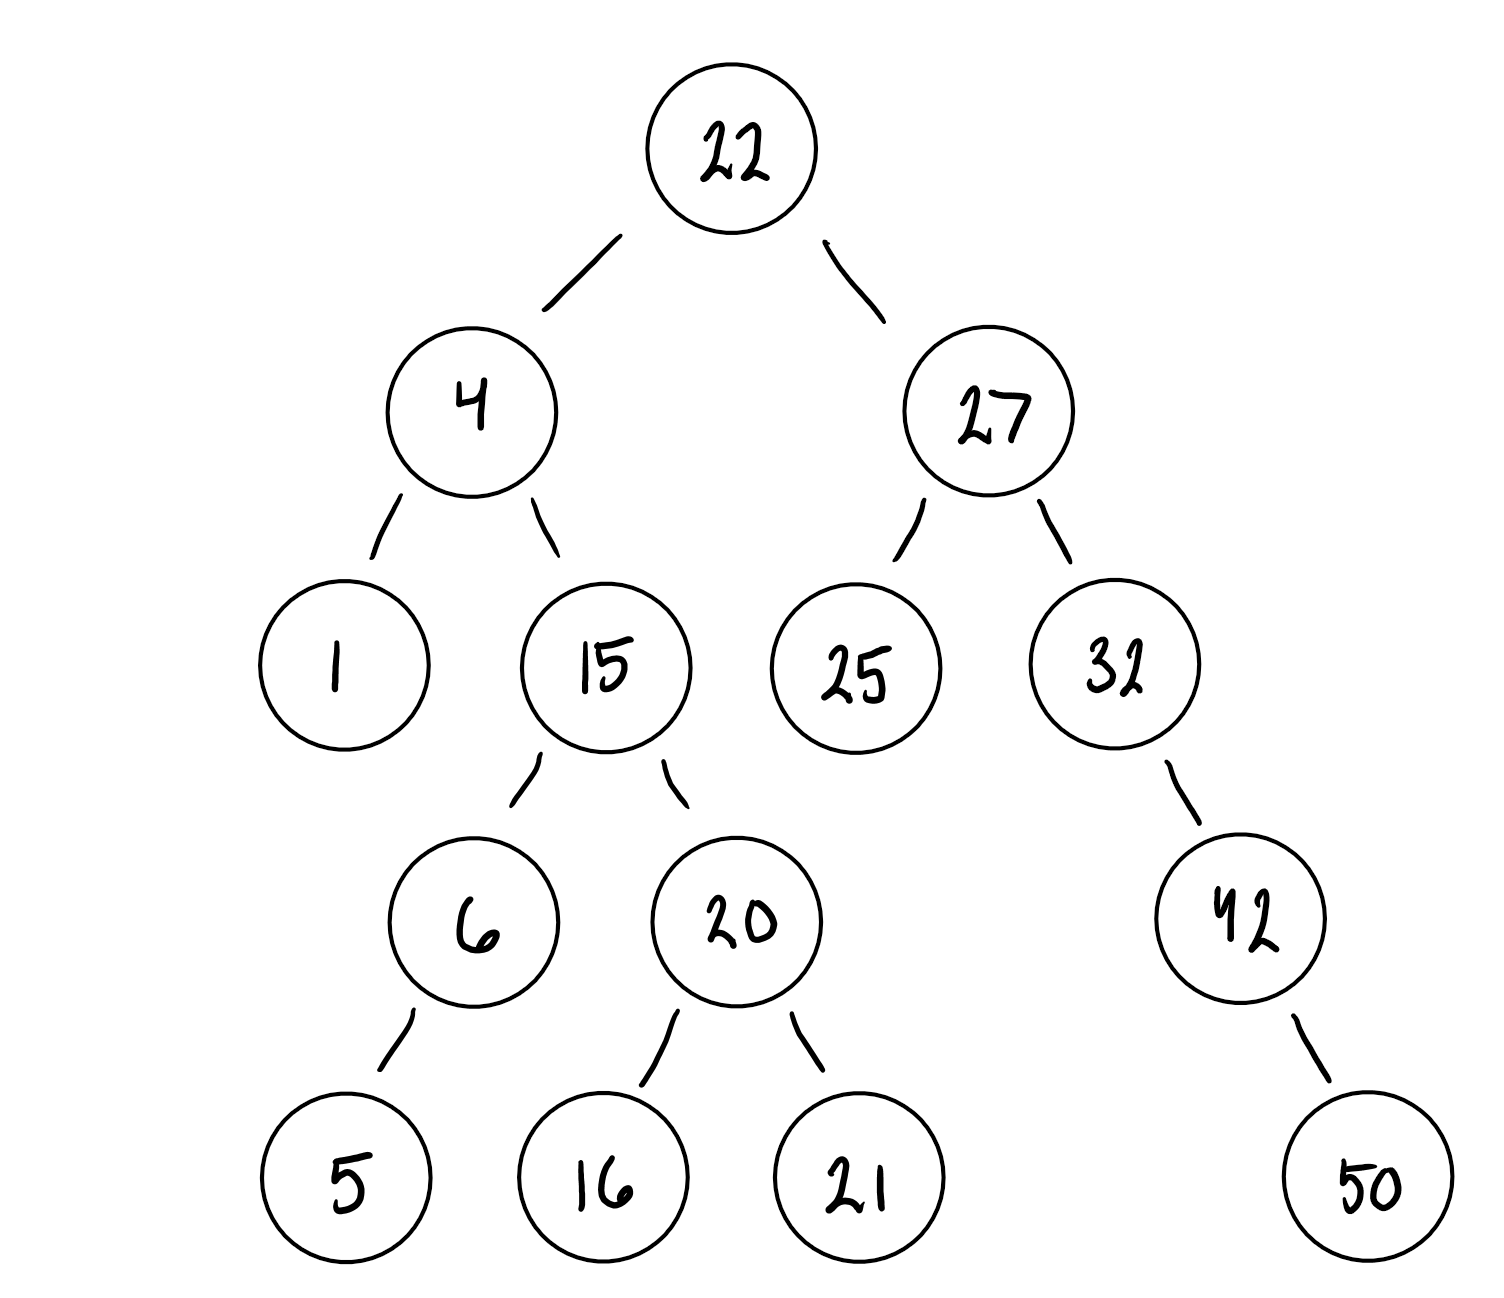
\includegraphics[scale=0.25]{Images/P1A1.PNG}
        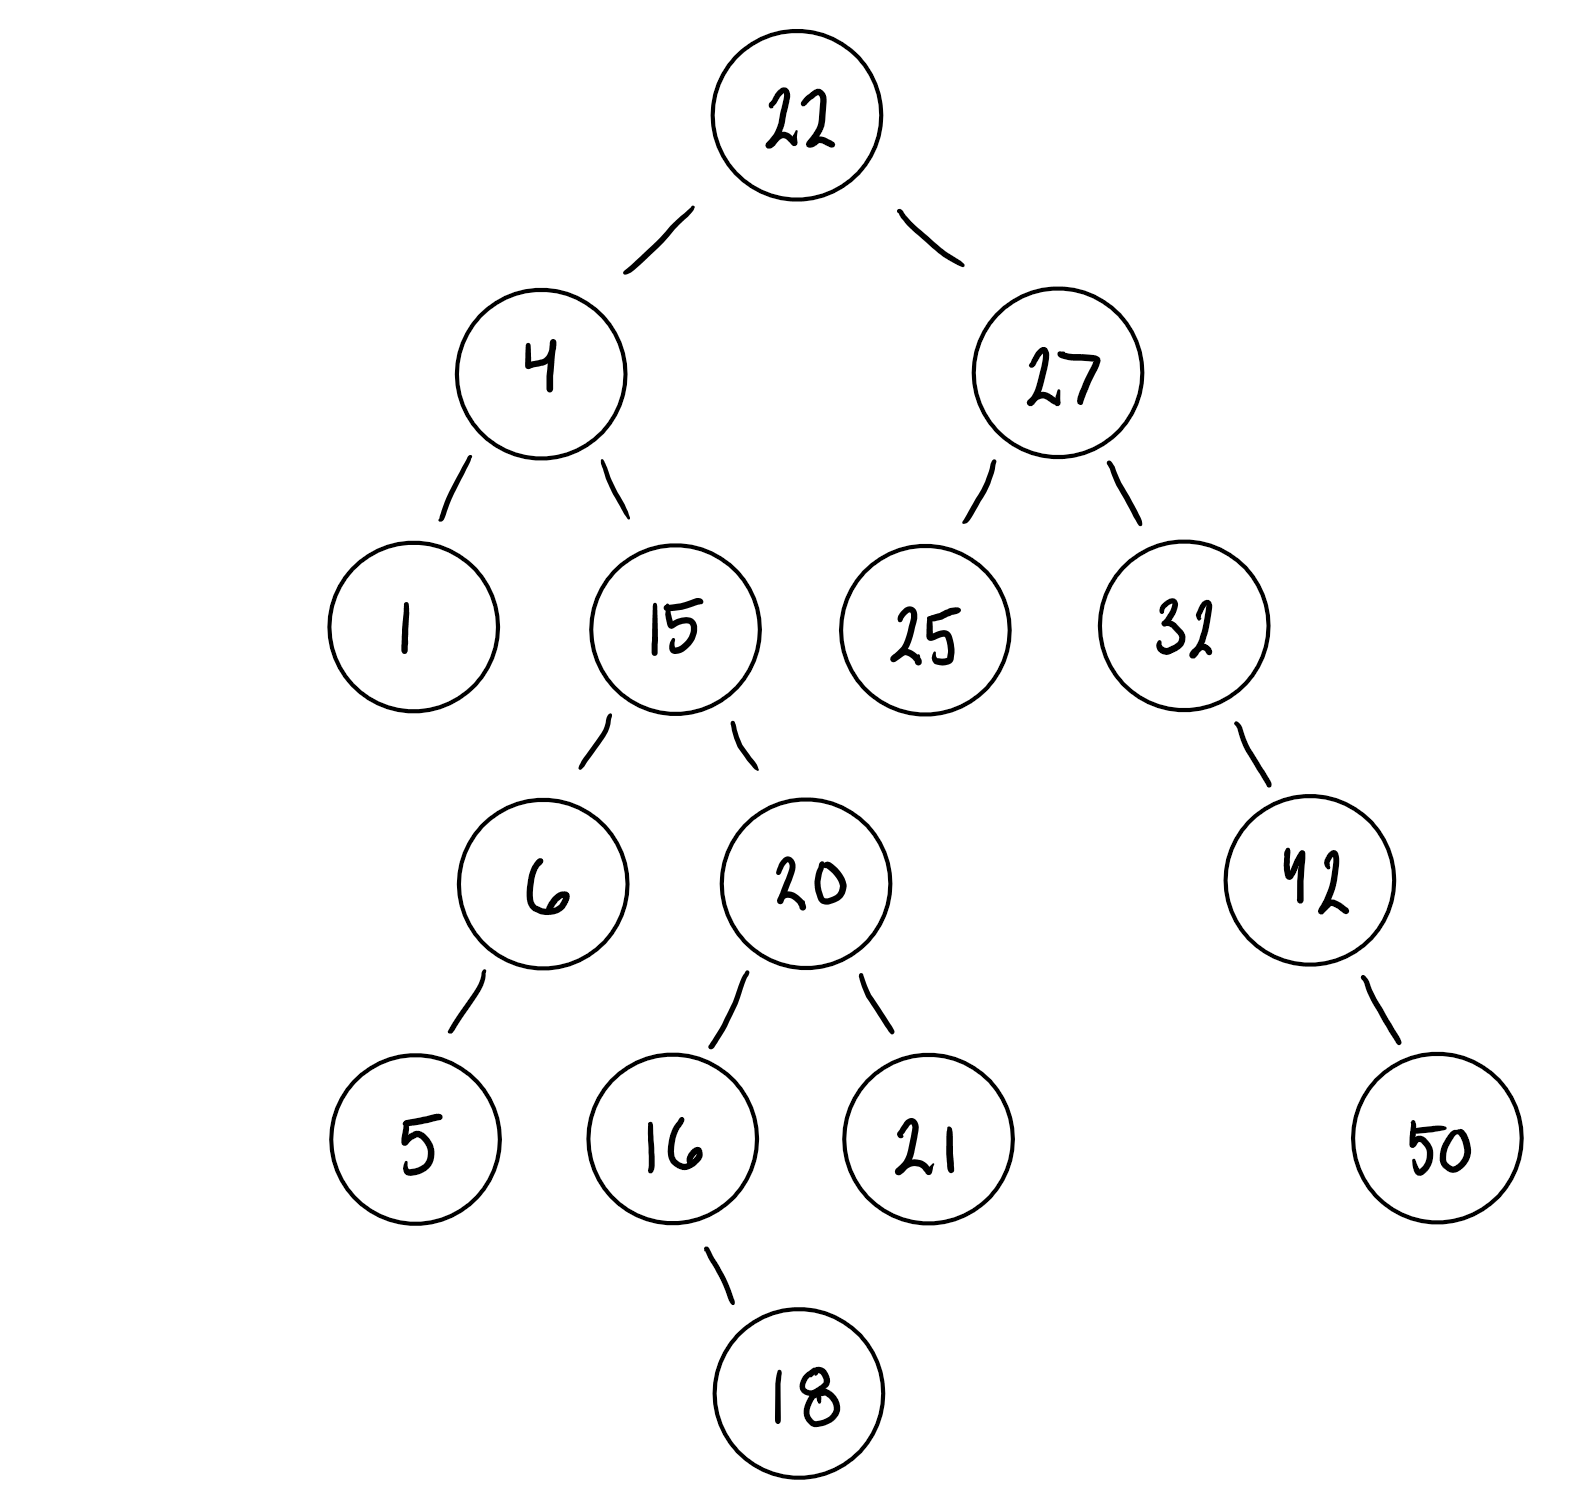
\includegraphics[scale=0.25]{Images/P1A2.PNG}
    \end{center}

    {\tt delete(5)}, {\tt insert(26)}:

    \begin{center}
        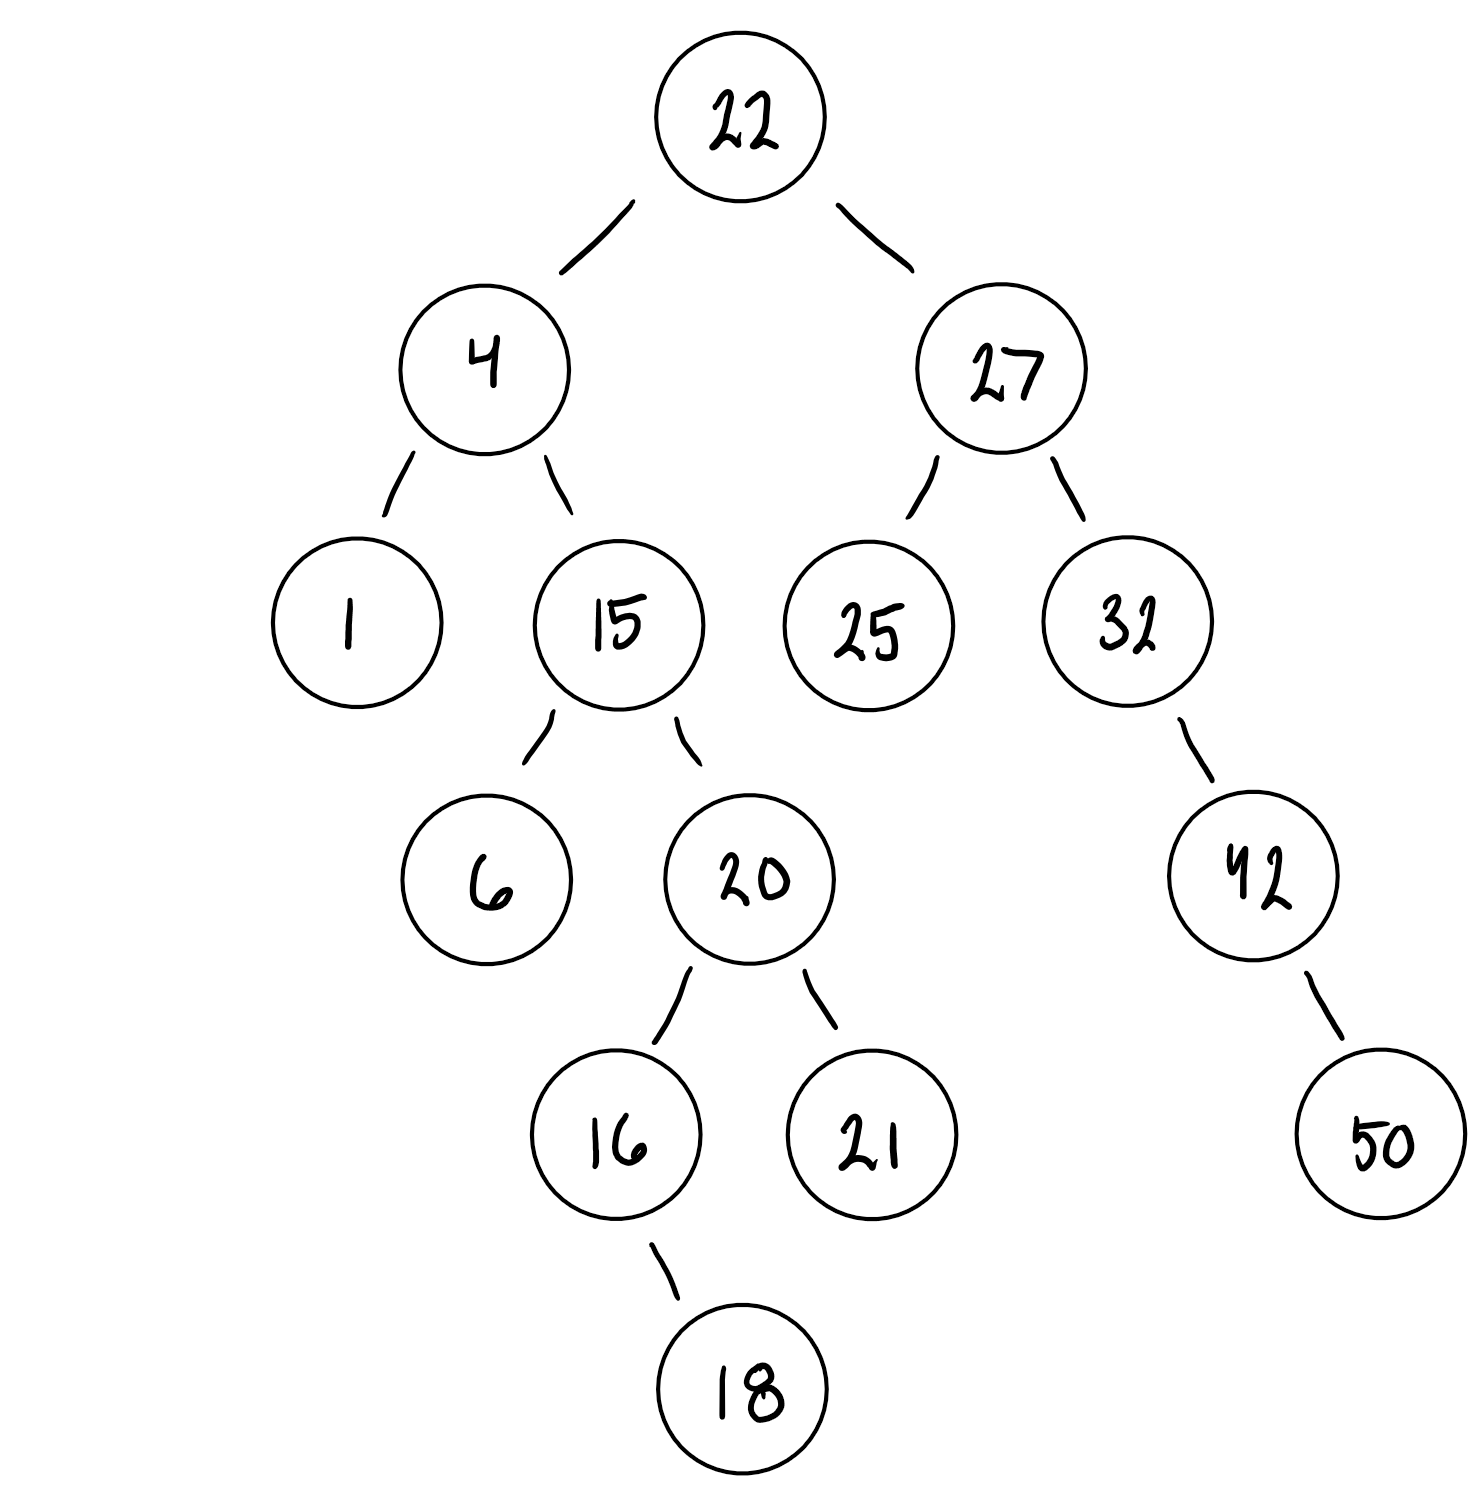
\includegraphics[scale=0.25]{Images/P1A3.PNG}
        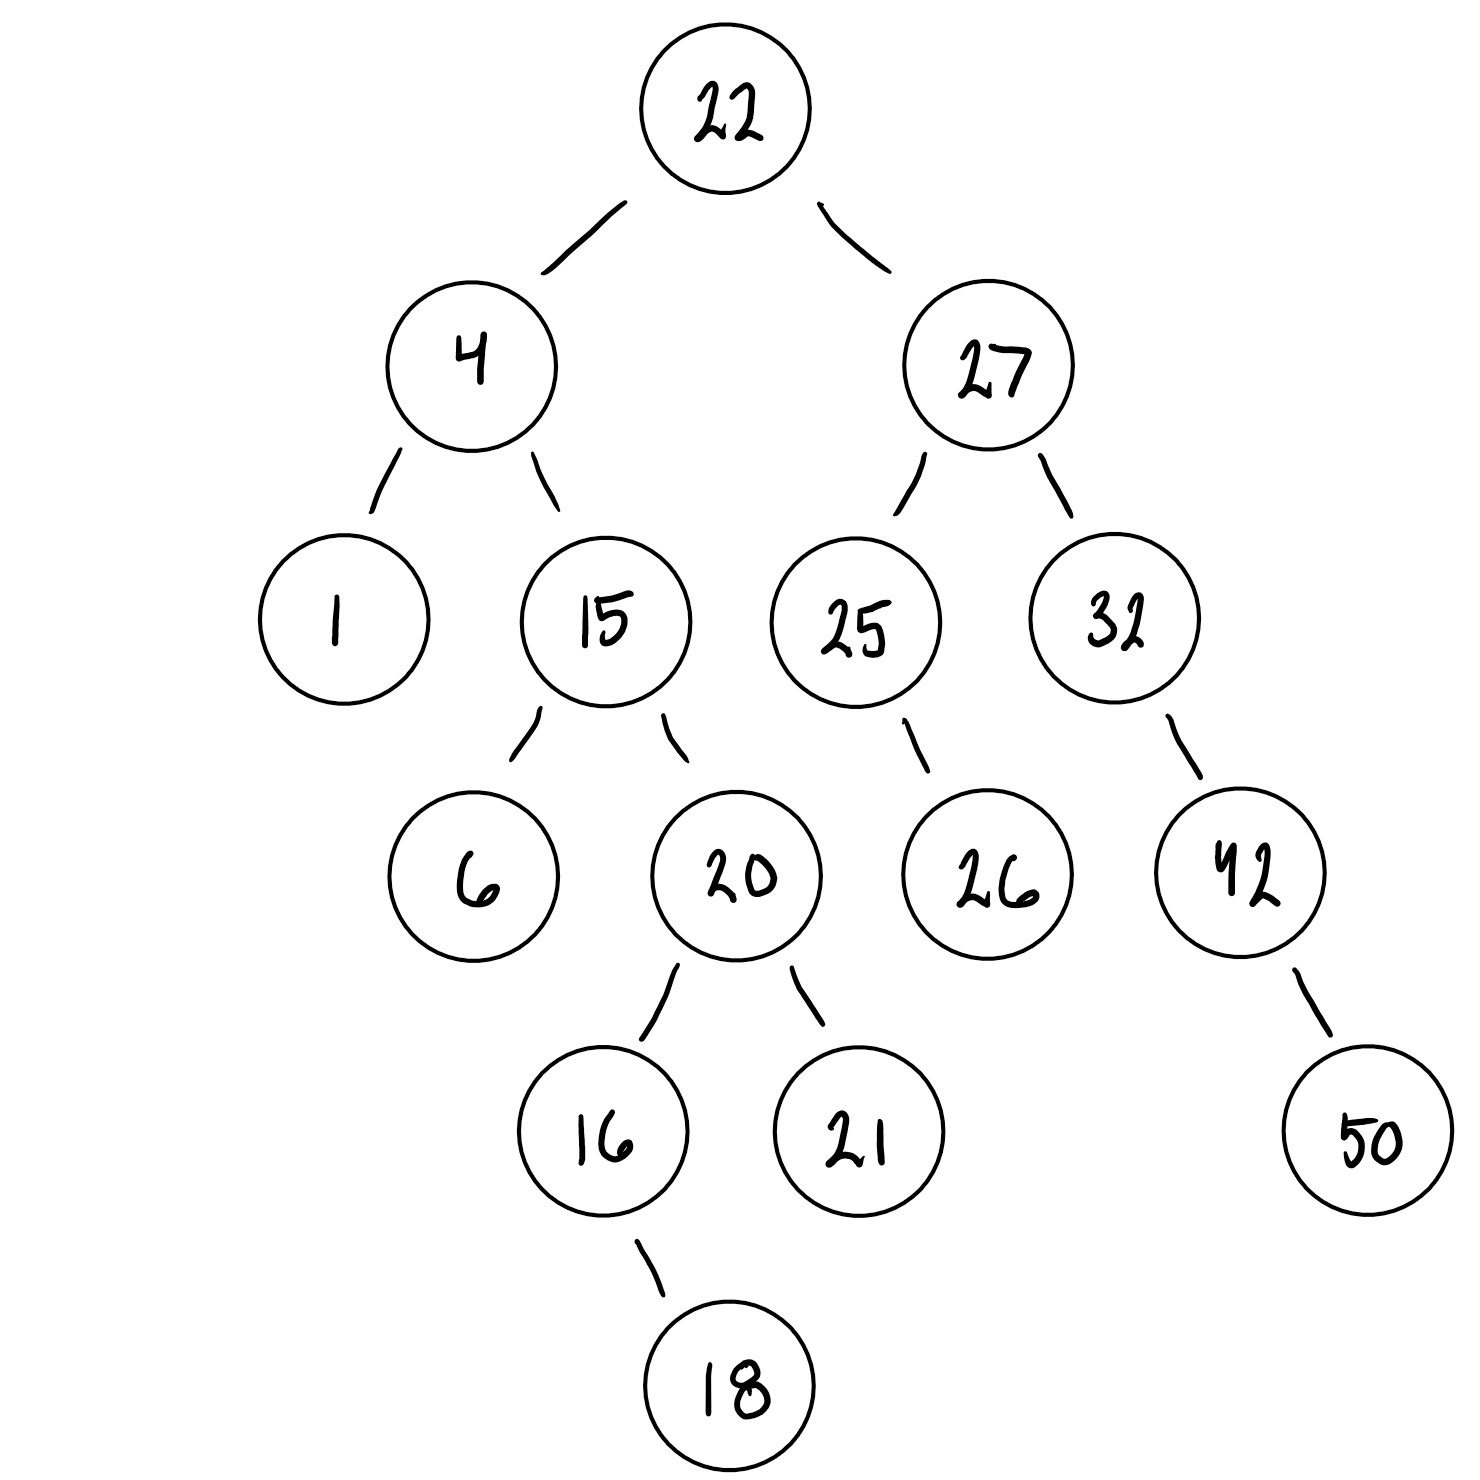
\includegraphics[scale=0.25]{Images/P1A4.PNG}
    \end{center}

    {\tt delete(32)}, {\tt delete(15)}:

    \begin{center}
        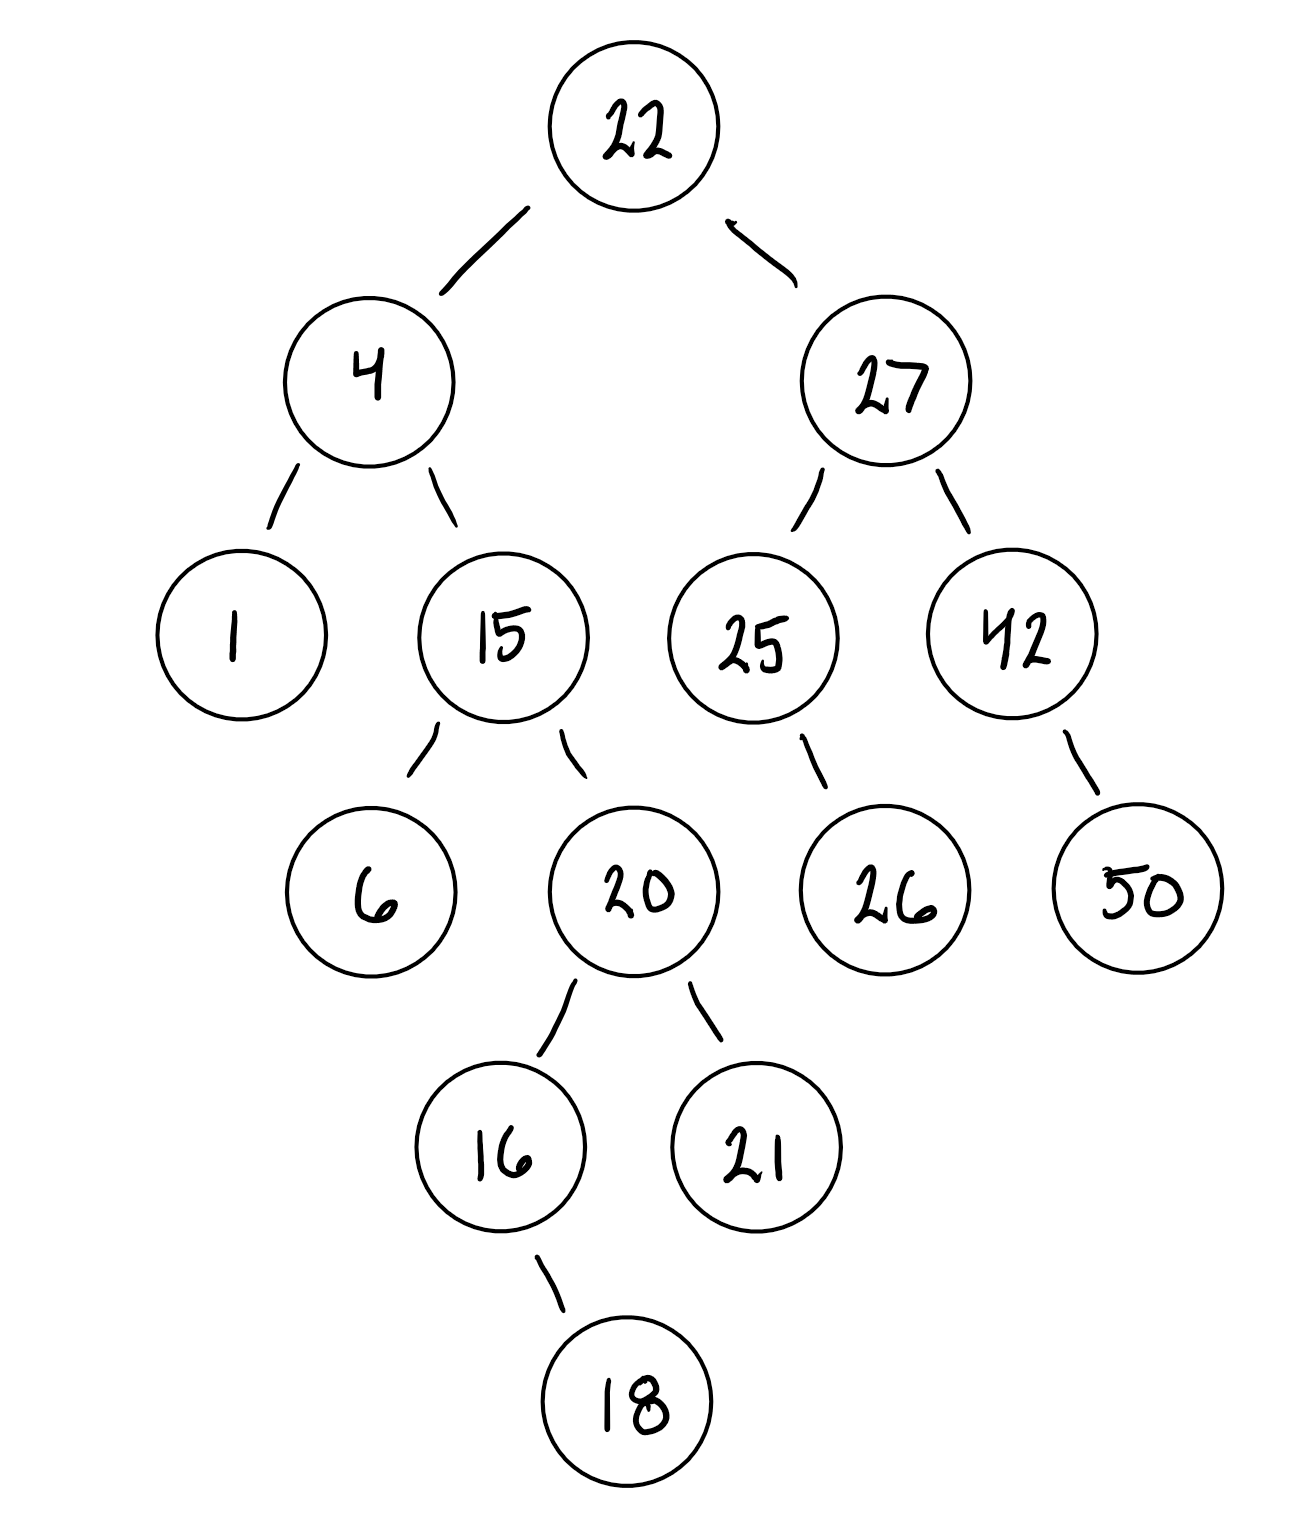
\includegraphics[scale=0.25]{Images/P1A5.PNG}
        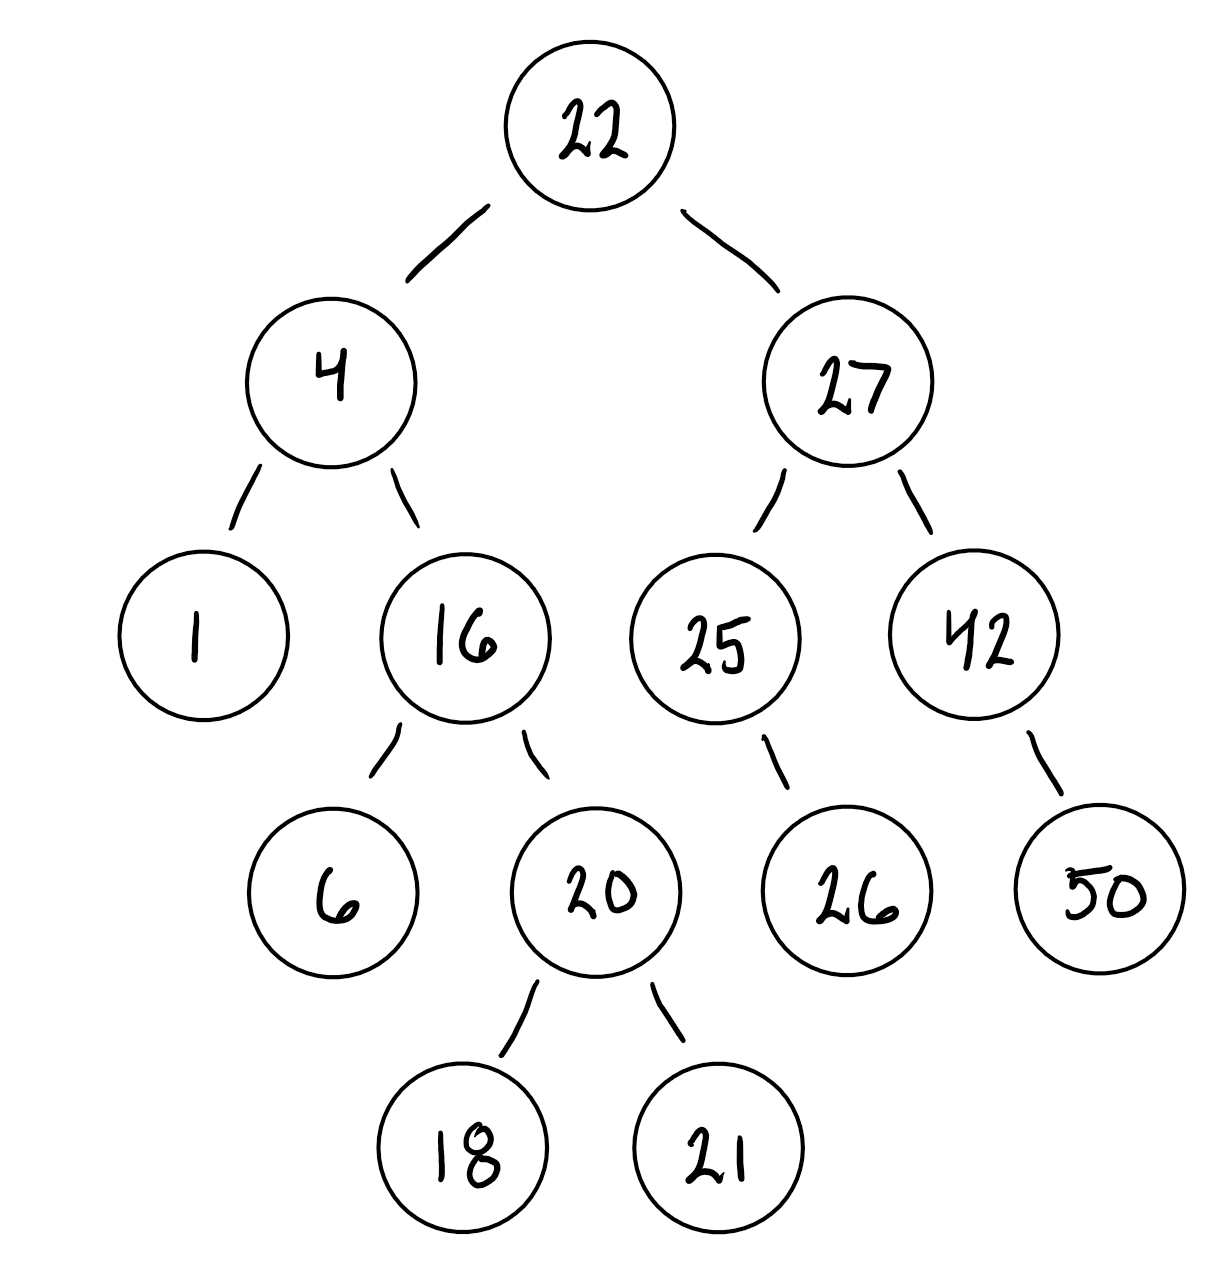
\includegraphics[scale=0.25]{Images/P1A6.PNG}
    \end{center}

\problempart In the original tree $ T $, the nodes with keys $ 4 $, $ 27 $,
    and $ 32 $ each have a skew equal to $ 2 \not\in \{-1, 0, 1 \} $ and
    therefore violates the AVL property.

\problempart Original tree $ T $ with root of rotation to be performed:

    \begin{center}
        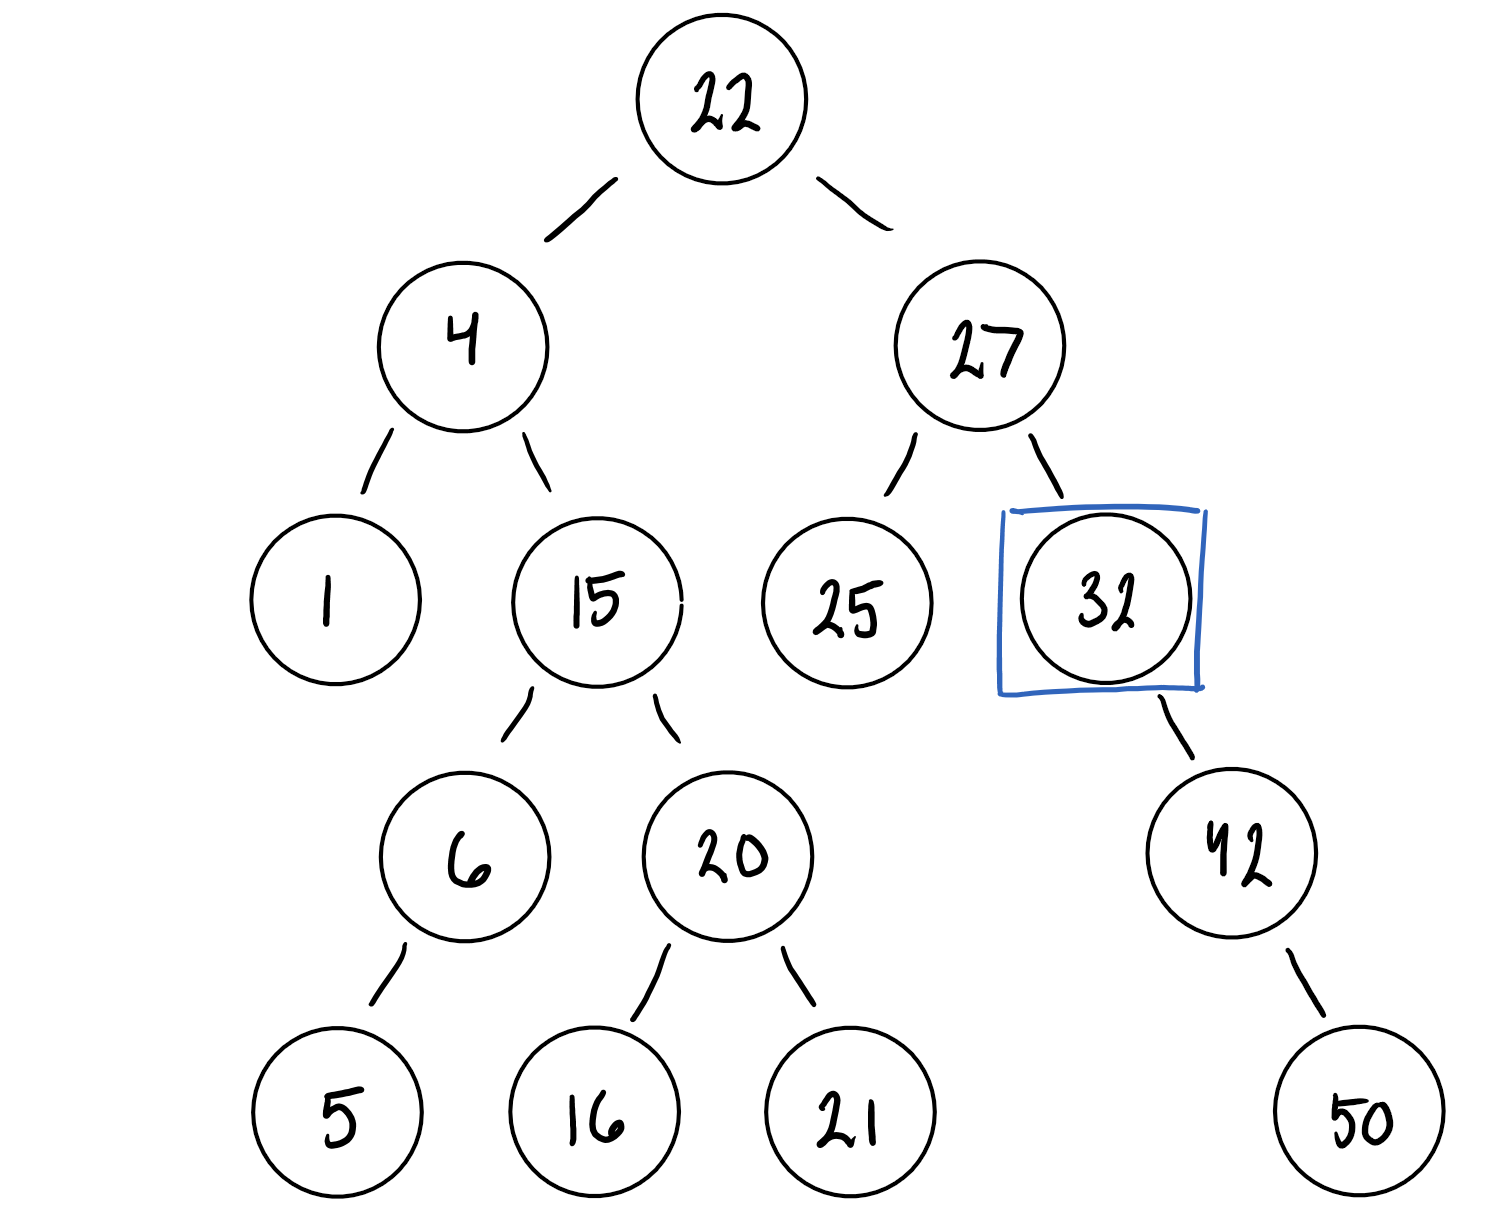
\includegraphics[scale=0.4]{Images/P1C1.PNG}
    \end{center}

    {\tt rotate\_left(32)}:

    \begin{center}
        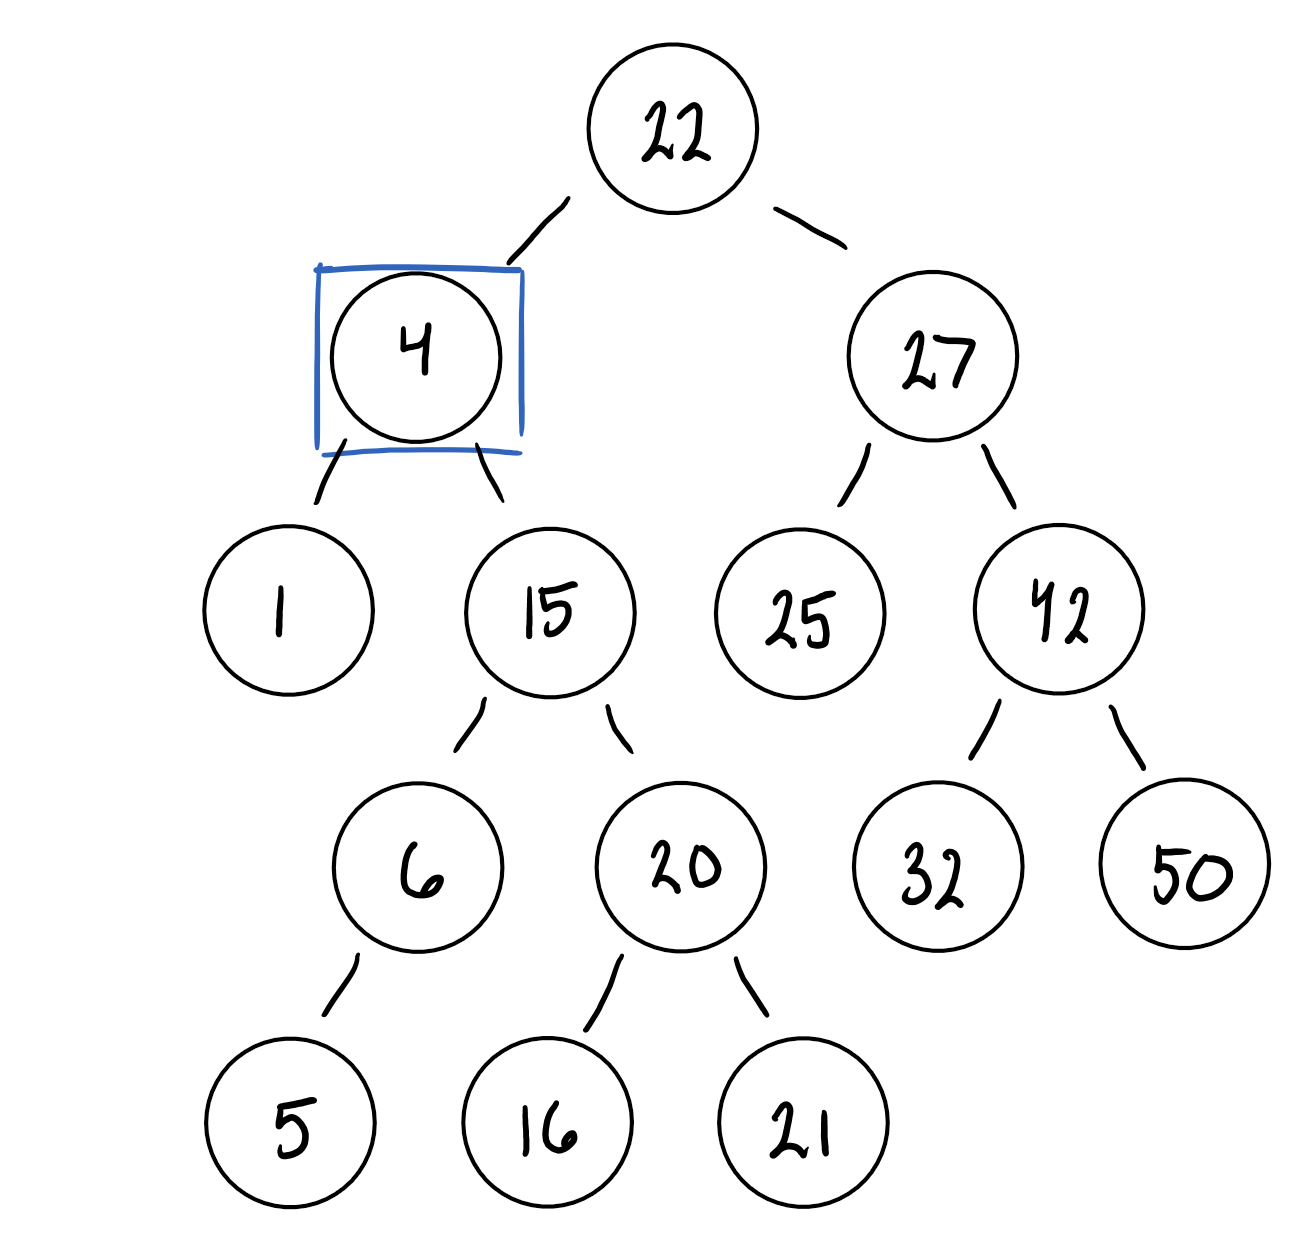
\includegraphics[scale=0.4]{Images/P1C2.PNG}
    \end{center}

    {\tt rotate\_left(4)}:

    \begin{center}
        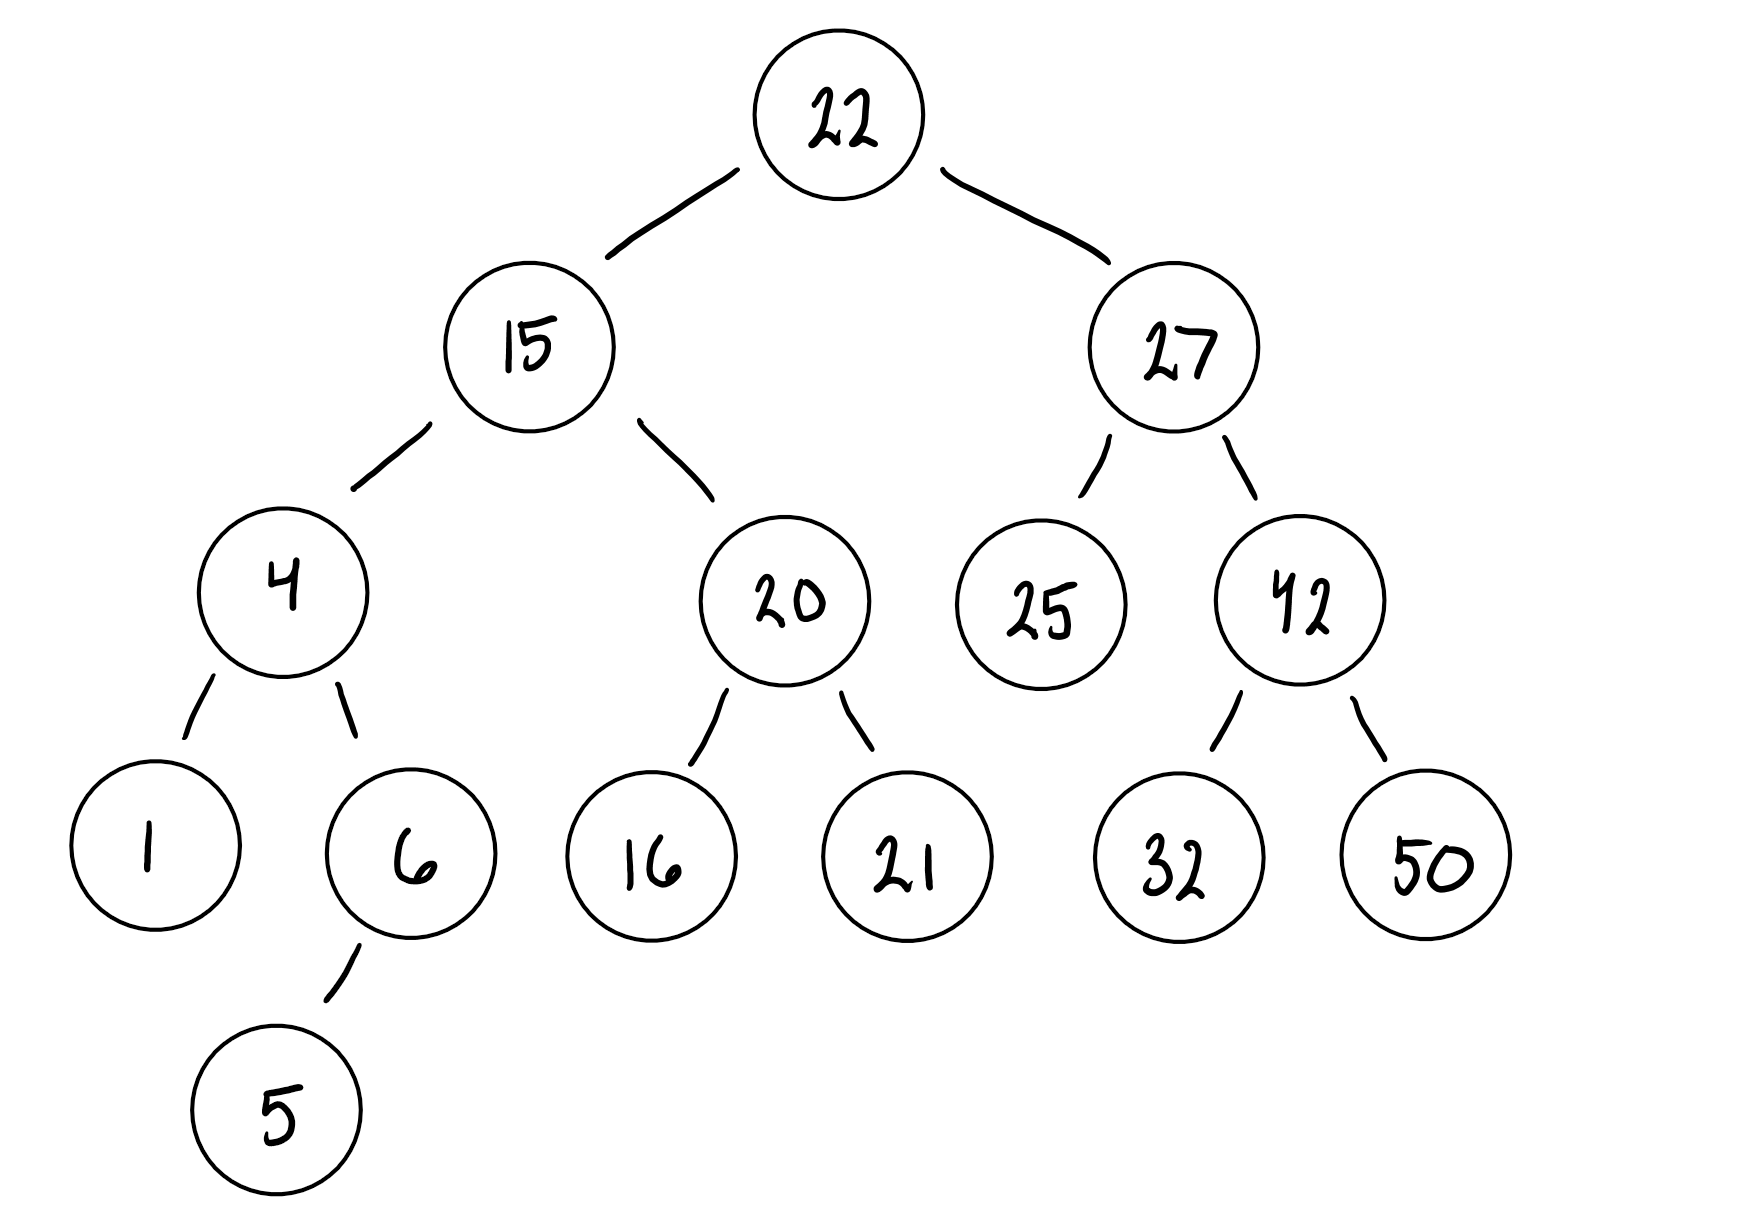
\includegraphics[scale=0.4]{Images/P1C3.PNG}
    \end{center}

\end{problemparts}

\newpage
\problem

\begin{problemparts}

\problempart {\bf Description}: This data structure/base has a single property
    \begin{itemize}
        \item {\tt fleeces}: An AVL tree that maintains a sorted set of
        fleeces based on the ascribed price (the key).
    \end{itemize}
    This data structure/base supports three methods
    \begin{itemize}
        \item {\tt add\_fleece(fleece)}: Perfoms an insert into the AVL tree
        {\tt fleeces} where {\tt fleece.price} is the key.
        \item {\tt modified\_find(price)}: This returns the fleece
        corresponding to the price key, it is exists, like a typical AVL
        find. If the key does not exist, the last visited fleece is returned
        instead.
        \item {\tt remove\_ten\_below(price)}: Performs a modified search
        (see below) in the AVL tree {\tt fleeces} for {\tt price}. Three
        cases are possible:
        \begin{itemize}
            \item Price is found: Return the fleece whose key is price and
            then call an AVL find-previous nine times, returning each located
            fleece. Then, for each returned fleece, call an AVL delete.
            \item Price is not found and the last visited fleece had a lower
            price: Return the fleece corresponding to the last visited node and
            then call an AVL find-previous nine times, returning each located
            fleece. Then, for each returned fleece, call an AVL delete.
            \item Price is not found and the last visited fleece has a higher
            price: Call an AVL find-previous ten times, returning each located
            fleece. Then, for each returned fleece, call an AVL delete.
        \end{itemize}
    \end{itemize}

    \smallbreak

    {\bf Correctness}: \begin{itemize}
        \item {\tt add\_fleece(fleece)}: This only involves calling an AVL
        add method which is assumed to correctly place the fleece within the
        AVL tree based on the key, which is the price. Thus, the fleece will
        be added correctly.
        \item {\tt modified\_find(price)}: This is exactly like an AVL find
        which is assumed to return the node associated with the key. However,
        instead of returning {\tt None} if the key is not found, it simply
        returns the last visited node which may be less than or greater than
        the price being searched for. However, given the BST property is in
        place in {\tt fleeces}, the last visited node can {\it only} be
        directly adjacent to the desired node if it were to exist.
        \item {\tt remove\_ten\_below(price)}: Given the modified find is
        guaranteed to return the fleece associated with the key or a fleece
        directly adjacent to a fleece with that key, there are only three cases
        \begin{itemize}
            \item Price is found: This fleece and the nine previous must be
            less than or equal to the specified price. An AVL find-previous
            is assumed to return the previous so if each returned fleece is
            fed into the find-previous nine times, the ten fleeces less than
            or equal to the specified price must be returned. 
            \item Price is not found and the last visited fleece had a lower
            price: Given the correctness of the modified find, this fleece
            must be the greatest fleece less than the specified price.
            Therefore, it and nine previous are the ten priciest fleeces less
            than the specified price. Proceed as in the last case.
            \item Price is not found and the last visited fleece had a higher
            price: Given the correctness of the modified find, this fleece
            must be the least fleece greater than the specified price.
            Therefore, its ten previous must be the ten priciest fleeces less
            than the specified price. Proceed as in the last case.
        \end{itemize}
        Then, an AVL delete will remove all the returned fleeces in all
        cases, which is assumed correct. Thus, the ten fleeces will be
        returned correctly.
    \end{itemize}

    \smallbreak

    {\bf Running Time}: \begin{itemize}
        \item {\tt add\_fleece(fleece)}: Simply an AVL add: $ O(\log n) $.
        \item {\tt modified\_find(price)}: Simply an AVL find, but keeping
        track of the last visited node (no extra work): $ O(\log n) $.
        \item {\tt remove\_ten\_below(price)}: In all cases, a single
        modified find takes place with $ O(\log n) $. Then, for the first two
        cases, nine subsequent AVL find-previous are called, each $ O(\log n
        ) $. In the third cases, ten instead of nine are called. Lastly, ten
        AVL deletes are performed, each $ O(\log n) $. This running time is
        worst case $ O(21 \log n) \in O(\log n) $.
    \end{itemize}

\problempart {\bf Description}: This data structure/base has a single
    property:
    \begin{itemize}
        \item {\tt clusters}: An AVL tree sorted by the location of the
        cluster. Each node in {\tt clusters} is also an AVL tree sorted by
        the print quality of the printer.
    \end{itemize}
    This data structure/base supports four methods:
    \begin{itemize}
        \item {\tt put\_online(printer)}: Performs an AVL find to determine
        if there are other printers located at the specified location. Two
        cases:
        \begin{itemize}
            \item Other printers exist at same location: Perform an AVL
            insert into the tree at this node, based on the quality key.
            \item No other printers exist at same location: Perform an AVL
            insert into the {\tt clusters} AVL tree based on location key.
            The node to insert is an AVL tree containing the single new
            printer.
        \end{itemize}
        \item {\tt take\_offline(printer)}: Performs an AVL find to locate
        the AVL tree in {\tt clusters} with the printer's location. Then,
        within the located AVL tree, an AVL delete is performed based on the
        printer's quality. If the AVL tree in {\tt clusters} is now empty,
        perform an AVL delete on {\tt clusters} based on the printers
        location.
        \item {\tt modified\_find(location)}: Performs an AVL find, but, if
        the specified location is not found, return the last visited node.
        This node will be directly adjacent to the desired node, but could be
        greater or less than. The returned node {\it may or may not} be the
        closest location to the desired location.
        \item {\tt best\_closest(location)}: Performs a modified AVL find to
        locate the location or a directly adjacent location. Three cases
        \begin{itemize}
            \item Location is found: Return the maximum quality printer
            within the AVL tree at that location.
            \item Location is not found and the returned location is greater:
            Call an AVL find-previous to get the directly adjacent location
            less than the location specified. Compare the relative distances.
            Take the closer and perform an AVL find-maximum on the AVL tree
            at that location.
            \item Location is not found and the returned location is less:
            Call an AVL find-next to the the directly adjacent location
            greater than the location specified. Compare the relative
            distances. Take the closer and perform an AVL find-maximum on the
            AVL tree at that location.
        \end{itemize}
    \end{itemize}

    \smallbreak

    {\bf Correctness}: \begin{itemize}
        \item {\tt put\_online(printer)}: AVL find will determine if the
        location-constant node exists (assumed correct).
        \begin{itemize}
            \item If node doesn't exist: AVL insert is performed to add a new
            node with an AVL tree with one node (assumed correct).
            \item If node exists: AVL insert is performed within that
            location-constant AVL tree (assumed correct).
        \end{itemize}
        Thus the printer will be added correctly.
        \item {\tt take\_offline(printe)}: AVL find (assumed correct) will
        determine the location-constant node to perform an AVL delete
        (assumed correct). An additional AVL delete (assumed correct) will be
        performed if the size of the AVL tree at the location becomes zero.
        Thus the printer will be removed correctly
        \item {\tt modified\_find(location)}: Same as argued in Part A. Note
        this also realizes that the returned node may not have the closest
        location if it is not the exact location searched for.
        \item {\tt best\_closest(location)}: \begin{itemize}
            \item If location found: Because of the correctness of the
            modified find, it must be the closest location since it is that
            location. The maximum quality printer within the cluster is
            returned using an AVL find-maximum (assumed correct). Note that
            this AVL tree is guaranteed to be non-empty from the
            specification of the {\tt take\_offline()}.
            \item If location not found: Returned location must be greater
            than or less than the desired location. The respective previous
            or next is found using the appropriate AVL find method (assumed
            correct). Since the returned location from the modified find is
            guaranteed to be directly adjacent, but may or may not be the
            closest. Compare the two locations and select the closest. These
            two must be closest given from the BST property. Therefore,
            perform in the same way as the last case with the selected node.
        \end{itemize}
        Thus the closest, highest quality printer is returned.
    \end{itemize}

    \smallbreak

    {\bf Running Time}: \begin{itemize}
        \item {\tt put\_online(printer)}: AVL find: $ O(\log n) $. And then
        an AVL insert to add to the found cluster (or create the cluster): $
        O(\log n) $. Total: $ O(2 \log n) \in O(\log n) $.
        \item {\tt take\_offline(printer)}: AVL find to find cluster: $
        O(\log n) $. Then AVL delete within cluster to find printer: $ O(\log
        n) $. Then, another possible AVL delete to remove empty cluster: $
        O(\log n) $. Note that the deletes will never both be $ O(\log n) $.
        Therefore, total running time: $ O(2 \log n) \in O(\log n) $.
        \item {\tt modified\_find(location)}: Same as in Part A: $ O(\log n) $.
        \item {\tt best\_closest(location)}: An AVL find to get cluster: $
        O(\log n) $. Then, at worst, an AVL find-previous/-next to get other
        adjacent location: $ O(\log n) $. Lastly, an AVL find-maximum within
        the cluster: $ O(\log n) $. Total: $ O(3 \log n) \in O(\log n) $.
    \end{itemize}

    Note: An AVL tree of heaps will be slightly more performant ($ O(1) $
    find-maximum instead of $ O(\log n) $) and support the same operations. I
    didn't realize this immediately, but the AVL tree of AVL trees still
    satisfies the question requirements.

\problempart {\bf Description}: This data structure/base will have one property
    \begin{itemize}
        \item {\tt letters}: An AVL tree whose key is the postmark date/time.
        Also contains information about the letter (like the sender).
    \end{itemize}
    This data structure/base will support two methods
    \begin{itemize}
        \item {\tt add(letter)}: This will perform an AVL insert into the
        letters AVL tree based on the postmark date/time. Will also add the
        sender information.
        \item {\tt at(k)}: This will perform an AVL find-minimum. Then, $k -
        1$ AVL find-next's. The last returned sender from the string of
        find-next's is then returned.
    \end{itemize}

    \smallbreak

    {\bf Correctness}: \begin{itemize}
        \item {\tt add(letter)}: Just an AVL insert assumed correct.
        \item {\tt at(k)}: AVL find-minimum (assumed correct) will give
        starting point for the $ k $ letters in postmark order. $ k - 1 $
        find-nexts will return the next $ k - 1 $ letters in postmark order.
        The last of the returned letters must be the $ k $th letter.
    \end{itemize}

    \smallbreak

    {\bf Running Time}: \begin{itemize}
        \item {\tt add(letter)}: Just an AVL insert: $ O(\log n) $.
        \item {\tt at(k)}: AVL find-minimum: $ O(\log n) $. Then, $ k - 1 $
        find-nexts each individually worst case $ O(\log n) $. The naive
        worst case is thus $ O(k \log n) $. This is fine for small $ k $.
        However, this is not the tightest bound. The $k - 1$ find next can be
        shown to actually be $ O(k) $ in aggregate. This is because a string
        of find-nexts is simply an in-order traversal of the AVL tree. As a
        result, at worst, if $ k = n $, then this traversal would be $ O(n) $
        not $ O(n \log n) $ as each node is hit exactly once. Therefore, on
        average, $ k $ find-nexts will be $ O(k) $. Therefore, the total
        running time is actually $ O(\log n + k) $ which is better than the
        naive bound.
    \end{itemize}

\end{problemparts}

\newpage
\problem

\begin{problemparts}

\problempart Since Python uses dynamic arrays, the {\tt add\_transaction}
    operation is amortized $ O(1) $, but could be worst-case $ O(n) $. The
    {\tt interval\_revenue} operation has to visit every transaction so it
    must be $ O(n) $.

\problempart Let $ m_i $ be an augmentation stored in the $i$th node within a
    given AVL tree. $ m_i $ represents the sum of all transactions included
    in the right and left subtrees of node $ i $ as well as the transaction
    within $ i $ itself. Let $ P(n) $ be the hypothesis that $ m_n $ stored
    in a node at height $n$ in a given AVL tree can be computed in $ O(1) $
    time.

    {\bf Base Case}: Let $ n = 0 $. That is, the node in which $ m_n $ is
    contained is a leaf. This means that the sum of the left and right
    subtrees is zero. Thus, $ m_n = t $, that is, the sum of all transactions
    is simply the value of the transaction at that node. Only one operation
    is required, therefore $ O(1) $ and the hypothesis $ P(n) $ is satisfied.

    {\bf Inductive Step}: Assume by induction that the inductive hypothesis
    is true for all nodes at height $ n $. More concretely, this means that
    the sums $m_n$ hold the sum of all transactions in their left and right
    subtrees (plus their own transaction) and that they were computed in
    constant time. Now, the sum $ m_{n + 1} $ is calculated by adding two
    sums from nodes at height $n$ and then adding their own transaction.
    Since both $m_n$ were computed in $ O(1) $ time and two additions is also
    $ O(1) $, this whole process takes $ O(1) $. Thus, the hypothesis is true
    for $ P(n + 1) $.

    Since the hypothesis holds for the base case and the inductive step, by
    induction, $m_n$ represents the sum of all transactions contained in any
    node's subtree and it is computed in $ O(1) $ time from bottom up.

    \smallbreak

    Since it was shown that the augmentation is computed in constant time
    from the bottom up for any node, and any {\tt insert} or {\tt delete}
    operations incur updates from the bottom up, this augmentation can be
    maintained in constant time for the AVL tree.

\problempart Let $ t_{1,i} $ and $ t_{2,i} $ be augmentations stored in the
    $i$th node within a given AVL tree. $ t_{1,i} $ represents the minimum
    transaction contained in the subtree rooted at node $i$ and $ t_{2,i} $
    is the maximum. Let $ P(n) $ be the hypothesis that $ t_{1,i} $ (or $
    t_{2,i} $, which is identical) stored in a node at height $ n $ in a
    given AVL tree can be computed in $ O(1) $ time.

    {\bf Base Case}: Let $ n = 0 $. That is, the node in which $ t_{1, n} $
    is contained is a leaf. Thus, $ t_{1, n} = t $, that is, the minimum of
    all transactions contained at this subtree is simply the value of the
    transaction at this node. Only one operation is required, therefore $
    O(1) $ and the hypothesis $ P(n) $ is satisfied.

    {\bf Inductive Step}: Assume by induction that the inductive hypothesis
    is true for all nodes at height $ n $. More concretely, this means that
    the minimums $ t_{1, n} $ hold the minimum of all transactions in their
    left and right subtrees (including their own transaction) and that they
    were computed in constant time. Now, the minimum $ t_{1,n+1} $ must
    either be the minimum of the left subtree, if it exists, or the
    transaction contained within the node at height $n + 1$, if the left
    subtree doesn't exist. Since the minimum of the left subtree was computed
    in $ O(1) $ time by the inductive assumption, this can be determined in $
    O(1) $ time and thus the inductive hypothesis $ P(n + 1) $ is true.

    Since the hypothesis holds for the base case and the inductive step, by
    induction, $ t_{1, n} $ (and $ t_{2,n} $, by symmetrical proof)
    represents the minimum (and maximum) of all transactions contained in any
    node's subtree and it is computed in $ O(1) $ time from the bottom up.

    \smallbreak
    
    Since it was shown that the augmentation is computed in constant time
    from the bottom up for any node, and any {\tt insert} or {\tt delete}
    operations incur updates from the bottom up, this augmentation can be
    maintained in constant time for the AVL tree.

\problempart {\bf Description}: If $ t_2 $ is less than the lower bound ($
    t_{1,i} $) stored on the given node or if $ t_1 $ is greater than the
    upper bound ($ t_{2,i} $) stored on the given node, the node and all
    of its descendants are outside of the desired range. Return 0.

    If $ t_1 $ is less than or equal to the lower bound ($t_{1,i}$) stored on
    the given node and $ t_2 $ is greater than or equal the upper bound
    ($t_{2,i}$) stored on the given node, the node and all its descendants
    are included in the desired range. Return the sum stored at that node.

    Recursive step: If the current element is within the desired range, add
    its value to a temporary sum. If the left node exists, recurse and add it
    to the temporary sum. If the right node exists, recurse and add it to the
    temporary sum.

    \smallbreak

    {\bf Correctness}: The first case is trivial as the two intervals do not
    overlap and therefore the sum in their intersection must be zero.

    The second case is equally trivial as the desired interval fully overlaps
    the current nodes interval. Given from Part C, the sum contained in that
    node must equal the sum of all of its descendants.

    The third case confirms the current node is within the desired range, then
    adds it ensuring no incorrect additions. Then the left and right trees are
    recursed if they exist.

\problempart If the desired range's lower bound is between a given node's
    minimum and its value and the desired range's upper bound is between a
    given node's value and maximum, then two recursions (one on the left 
    subtree and one on the right) are required. However, after this case,
    there are only two possibilities for each individual recursion. WLOG,
    take the left subtree recursion:
    \begin{itemize}
        \item The desired range's lower bound is between the node's minimum
        and its value: A recursion to the left is required. However, given
        the established previous recursion above, the upper bound of the
        desired range must be greater than the maximum of the current node.
        Therefore, no right recursion is necessary, just return the sum of
        that right subtree.
        \item The desired range's lower bound is between the node's value and
        its maximum: Only a recursion to the right is required.
    \end{itemize}
    Any subsequent recursion will follow this pattern as well since one bound
    is guaranteed to be beyond either the maximum or minimum. Therefore, if
    this particular case is hit, it will only occur once.

\problempart Given the answer from Part E, although it appears that there is
    a branching factor of two, in reality, that will only occur once and thus
    the real branching factor is one. Furthermore, each branching roughly
    halves the problem size given the BST-AVL property. Lastly, each
    iteration only does constant comparisions. The recurrence is given
    $$ T(n) = T(n/2) + 1 $$
    By the second case of the Master Theorem, this is $ O(\log n) $.

\problempart Submit your implementation to {\small\url{alg.mit.edu/PS4}}
\end{problemparts}

\end{problems}

\end{document}

